%!TEX root = article.tex
We report the proofs of the different propositions (\autoref{sec:proofs}), an instantiation of online Sinkhorn for discrete measures (\autoref{sec:sinkhorn_discrete}), and a supplementary experiment (\autoref{sec:supp_exp}).

\section{Proofs}\label{sec:proofs}

We first introduce two useful known lemmas, and prove the propositions in their order of appearance.

\subsection{Useful lemmas}

First, under \autoref{ass:lip}, we note that the soft $C$-transforms are
 uniformly contracting on the distribution space $\Pp(\Xx)$. This is clarified
 in the following lemma, extracted from \citet{vialard2019elementary},
 Proposition 19. We refer the reader to the original references for proofs.

\begin{lemma}\label{lemma:contractance}
    Unser \autoref{ass:lip}, let $\kappa = 1 - \exp(-L
    \textnormal{diam}(\Xx))$. For all $\hat \alpha \in \Pp(\Xx)$ and $\hat \beta \in
    \Pp(\Xx)$, for all $f, f', g, g' \in \Cc(\Xx)$,
    \begin{equation}
        {\Vert \Ctrans{f'}{\hat \alpha} - 
        \Ctrans{f'}{\hat \alpha} \Vert}_{\var} \leq \kappa {\Vert f - f' \Vert}_{\var},
        \quad
        {\Vert \Ctrans{g}{\hat \beta} - 
        \Ctrans{g'}{\hat \beta} \Vert}_{\var} \leq \kappa {\Vert g - g' \Vert}_{\var}.
    \end{equation}
\end{lemma}

We will also need a uniform law of large numbers for functions. The following lemma is a consequence of Example 19.7 and
Lemma 19.36 of \citet{van_der_vaart_asymptotic_2000}, and is copied in Lemma B.6 in \citet{mairal_stochastic_2013}.

\begin{lemma}\label{lemma:lln}
    Under \autoref{ass:lip}, let $(f_t)_t$ be an i.i.d sequence in $\Cc(\Xx)$,
    such that $\EE[f_0] = f \in \Cc(\Xx)$. Then there exists $A > 0$ such that, for all $n > 0$,
    \begin{equation}
        \EE \sup_{x \in \Xx} | \frac{1}{n} \sum_{i=1}^n f_i(x) - f(x) |
        \leq \frac{A}{\sqrt{n}}.
    \end{equation}
\end{lemma}
Finally, we need a result on running averages using the sequence ${(\eta_t)}_t$. The following result stems from a simple Abel transform of the law of large number, and is established by \citet{mairal_stochastic_2013}, Lemma B.7.

\begin{lemma}\label{lemma:running}
    Let $(\eta_t)_t$ be a sequence of weights meeting \autoref{ass:weights}. Let
    $(X_t)_t$ be an i.i.d sequence of real-valued random variables with existing
    first moment $\EE[X_0]$. We consider the sequence ${(\bar X_t)}_t$ defined
    by $\bar X_0 \triangleq X_0$ and 
    \begin{equation}
        \bar X_t \triangleq (1 - \eta_t) \bar X_{t-1} + \eta_t X_t.
    \end{equation}
    Then $\bar X_t \to_{t \to \infty} \EE[X_0]$.
\end{lemma}

\subsection{Proof of \autoref{prop:markov}}

\begin{proof}
    We use Theorem 1 from \citet{diaconis_iterated}. For this, we simply note
    that the space $\Cc(\Xx) \times \Cc(\Xx)$ in which the chain ${x_t
    \triangleq (f_t, g_t)}_t$, endowed with the metric $\rho((f_1, g_1), (f_2,
    g_2)) = \Vert f_1 - f_2 \Vert_{\var} + \Vert g_1 - g_2 \Vert_{\var}$, is
    complete and separable (the countable set of polynomial functions are dense in this space, for example).
    We consider the operator $A_{\theta} \triangleq \Ctrans{\Ctrans{\cdot}{\hat
    \alpha}}{\hat \beta}$. $\theta \triangleq (\hat \alpha, \hat \beta)$ denotes
    the random variable that is sampled at each iteration. We have the following
    recursion:
    \begin{equation}
        x_{t+2} = A_{\theta_t}(x_t).
    \end{equation}
    
    From \autoref{lemma:contractance}, for all $\hat \alpha \in \Pp(\Xx)$, $\hat \beta \in \Pp(\Xx)$, $A_{\theta}$
    with $\theta = (\hat \alpha, \hat \beta)$ is contracting, with module
    $\kappa_\theta < \kappa < 1$. Therefore
    \begin{equation}
        \int_{\theta} \kappa_\theta \d \mu(\theta) < 1, \qquad \int_{\theta}
         \log \kappa_\theta \d \mu(\theta) < 0.
    \end{equation}
    Finally, we note, for all $f \in \Cc(\Xx)$
    \begin{equation}
        \Vert \Ctrans{\Ctrans{f}{\hat \alpha}}{\beta} \Vert_{\infty} 
        \leq \Vert f \Vert_\infty + 2 \max_{x,y \in \Xx} C(x, y),
    \end{equation}
    therefore $\rho(A_\theta(x_0), x_0) \leq 2 \Vert x_0 \Vert_\infty + 2
    \max_{x,y \in \Xx} C(x, y)$ for all $\theta \ (\hat \alpha, \hat \beta)$.
    The regularity condition of the theorem are therefore met. Each of the
    induced Markov chains ${(f_{2t}, g_{2t})}_t$ and ${(f_{2t + 1}, g_{2t +
    1})}_t$ has a unique stationary distribution. These stationary distributions
    are the same: the stationary distribution is independent of the
    initialisation and both sequences differs only by their initialisation.
    Therefore ${(f_{t}, g_{t})}_t$ have a unique stationary distribution
    $(F_\infty, G_\infty)$.
\end{proof}

\subsection{Proof of \autoref{eq:deterministic}}

The \enquote{slowed-down} Sinkhorn iterations converge toward an optimal
potential couple, up to a constant factor: this stems from the fact that we
apply contractions in the space $(\Cc(\Xx), {\Vert\cdot\Vert}_{\var})$ with a
contraction factor that decreases sufficiently slowly.

\begin{proof}
    We write ${(f_t, g_t)}_t$ the sequence of iterates. Given a pair of optimal potentials 
    $(f^\star, g^\star)$, we write $u_t \triangleq f_t - f^\star$, $v_t \triangleq g_t - g^\star$,
    $u_t^T \triangleq \Ctrans{f_t}{\alpha} - g^\star$ and $v_t^T \triangleq \Ctrans{g_t}{\alpha} - f^\star$.
    For all $t > 0$, we observe that 
    \begin{align}
        \max u_{t+1} &= - \log \min \exp(-u_{t+1}) \\
        &= - \log \big( \min \big( (1 - \eta_t) \exp(-u_{t}) + \eta_t 
        \exp(-v_t^T) \big) \big)\\
        &\leq - \log \big( (1 - \eta_t) \min \exp(-u_{t}) + \eta_t 
        \min \exp(-v_t^T) \big)\\
        &\leq - (1 - \eta_t) \log \min \exp(-u_{t}) -  \eta_t \log \min
         \exp(-v_t^T) \\
         &= (1 - \eta_t) \max u_t  + \eta_t \max v_t^T,
    \end{align}
    where we have used the algorithm recursion on the second line, $\min f + g \geq \min f + \min g$
     on the third line and Jensen inequality on the fourth line. Similarly
    \begin{equation}
        \min u_{t+1} \geq (1 - \eta_t) \min u_t  + \eta_t \min v_t^T,
    \end{equation}
    and mirror inequalities hold for $v_t$. Summing the four inequalities, we obtain
    \begin{align}\label{eq:et}
        e_{t+1} &\triangleq \Vert u_{t+1} \Vert_{\var} + \Vert v_{t+1} \Vert_{\var} \\ 
        &= \max u_{t+1} - \min u_{t+1} + \max v_{t+1} - \min v_{t+1} \\
        &\leq
        (1 - \eta_t) ( \Vert u_t \Vert_{\var} + \Vert v_t \Vert_{\var})
        + \eta_t ( \Vert u_t^T \Vert_{\var} + \Vert v_t^T \Vert_{\var}), \\
        &\leq
        (1 - \eta_t) ( \Vert u_t \Vert_{\var} + \Vert v_t \Vert_{\var})
        + \eta_t \kappa ( \Vert u_t \Vert_{\var} + \Vert v_t \Vert_{\var}),
    \end{align}
    where we use the contractance of the soft-$C$-transform, that guarantees that
    there exists $\kappa < 1$ such that $\Vert v_t^T\Vert_{\var} \leq \kappa \Vert
    v_t\Vert_{\var}$ and $\Vert u_t^T\Vert_{\var} \leq \kappa \Vert
    u_t\Vert_{\var}$ \citep{peyre2019computational}.

    Unrolling the recursion above, we obtain
    \begin{equation}
        \log e_t = \sum_{s=1}^t \log(1 - \eta_t (1 - \kappa)) + \log(e_0) \to - \infty,
    \end{equation}
    provided that $\sum \eta_t = \infty$. The proposition follows.
\end{proof}

\subsection{Proof of \autoref{prop:convergence_bis}}

\begin{proof}
For discrete realizations $\hat \alpha$ and $\hat \beta$, we define the perturbation terms
\begin{equation}
    \epsilon_{\hat \beta}(\cdot) \triangleq
    f^\star - \Ctrans{g^\star}{\hat \beta} ,\qquad
    \iota_{\hat \alpha}(\cdot) \triangleq 
    g^\star - \Ctrans{f^\star}{\hat \alpha},
\end{equation}
so that the updates can be rewritten as
\begin{align}
    \exp(-f_{t+1} + f^\star) &= (1 - \eta_t)
    \exp(-f_{t} + f^\star)
    + \eta_t \exp(-\Ctrans{g_t}{\hat \beta_t} 
    +\Ctrans{g^\star}{\hat \beta_t} + \epsilon_{\hat \beta_t}) \\
    \exp(-g_{t+1} + g^\star) &= (1 - \eta_t)
    \exp(-g_{t} + g^\star)
    + \eta_t \exp(-\Ctrans{f_t}{\hat \alpha_t} 
    +\Ctrans{f^\star}{\hat \alpha_t} + \iota_{\hat \alpha_t}).
\end{align}
We denote $u_t \triangleq -f_{t} + f^\star$, $v_t \triangleq -g_{t} + g^\star$, $u_t^T \triangleq
\Ctrans{f_t}{\hat \beta_t} - \Ctrans{f^\star}{\hat \beta_t}$, $v_t^T \triangleq
\Ctrans{g_t}{\hat \beta_t} - \Ctrans{g^\star}{\hat \beta_t}$. Reusing the same
derivations as in the proof of \autoref{eq:deterministic}, we obtain
    \label{eq:pre_ineq_var}
    \begin{align}
    \Vert u_{t+1} \Vert_{\var} &\leq
    (1 - \eta_t) \Vert u_t \Vert_{\var}
    \\
    &\phantom{=}+ \eta_t \log \big( \max_{x, y \in \Xx}
    \exp(\epsilon_{\hat \beta_t}(x) 
    - \epsilon_{\hat \beta_t}(y)) \exp(v_t^T(x) - v_t^T(y)) \big) \\ 
    &\leq
    (1 - \eta_t) \Vert u_t \Vert_{\var}
    + \eta_t \Vert v_t^T \Vert_{\var}
    + \eta_t \Vert \epsilon_{\hat \beta_t} \Vert_{\var},
\end{align}
where we have used $\max_x f(x) g(x) \leq \max_x f(x) \max_x f(x)$ on the second line. Therefore,
using the contractance of the soft $C$-transform,
\begin{equation}
    \label{eq:ineq_var}
    e_{t+1} \leq 
    (1 - \tilde \eta_t) e_t
    +  \frac{\tilde \eta_t}{1 -\kappa}
    ({\Vert \epsilon_{\hat \beta_t} \Vert}_{\var} + 
    {\Vert \iota_{\hat \alpha_t} \Vert}_{\var}),
\end{equation}
where we set $e_t \triangleq \Vert u_t \Vert_{\var} + \Vert v_t \Vert_{\var}$,
$\tilde \eta_t = \eta_t (1-\kappa)$ and $\kappa$ is set to be the biggest
contraction factor over all empirical realizations $\hat \alpha_t$, $\hat
\beta_t$ of the distributions $\alpha$ and $\beta$. It is upper bounded by $1 -
e^{- L\text{diam}(\Xx)}$, thanks to \autoref{ass:lip} and
\autoref{lemma:contractance}.

The realizations $\hat \beta_t$ and $\hat \alpha_t$
are sampled according to the same distribution $\hat \alpha$ and $\hat \beta$. We
define the sequence $r_t$ to be the running average of the variational norm of the
(functional) error term:
\begin{equation}
    r_{t+1} \triangleq (1 - \tilde \eta_t) r_t + \frac{\tilde \eta_t}{1 - \kappa}
    ({\Vert \epsilon_{\hat \beta_t} \Vert}_{\var} + 
    {\Vert \iota_{\hat \alpha_t} \Vert}_{\var}).
\end{equation}
We thus have, for all $t > 0$, $e_t \leq r_t$. Using \autoref{lemma:running}, the sequence $(r_t)_t$
converges towards the scalar expected value
\begin{equation}\label{eq:r_infty}
    r_\infty \triangleq \frac{1}{1 - \kappa} \EE_{\hat \alpha, \hat \beta}[{\Vert \epsilon_{\hat \beta} \Vert}_{\var}
    + {\Vert \iota_{\hat \alpha} \Vert}_{\var}] > 0.
\end{equation}
We now relate $r_\infty$ to the number of samples $n$ using
a uniform law of large number result on parametric functions.

We now write $\hat \beta = \hat \beta_n$ to make explicit the dependency of the
quantities on the batch size $n$. We choose $g^\star = g^\star_0$ such that
$\max_{x \in X} g^\star_0(x) = 0$ without loss of generality.

Using \autoref{lemma:lln}, we bound the quantity
\begin{align}
    E_n &\triangleq \EE_{\hat \beta_n} {\Vert \exp(-\Ctrans{g^\star}{\beta})
    - \exp(-\Ctrans{g^\star}{\hat \beta_n}) \Vert}_{\infty} \\
    &= \EE_{Y_1, \dots Y_n \sim \beta} 
    \sup_{x \in \Xx}
     \Big| \frac{1}{n} \sum_{i=1}^n \exp(g^\star(Y_i)) - C(x, Y_i)) \\
      &\phantom{=}\qquad\qquad\qquad\quad- \EE_{Y \sim \beta}[\exp(g^\star(Y)) - C(x, Y)] \Big| \\
      &= \EE \sup_{x \in \Xx} | \frac{1}{n} \sum_{i=1}^n \phi_i(x) - \phi(x) | ,
\end{align}
where we have defined $\phi_i: x \to \exp(g^\star(Y_i) - C(x, Y_i))$ and set
$\phi$ to be the expected value of each $\phi_i$. The compactness of $\Xx$
ensures that the functions  are square integrable and uniformly bounded.
\autoref{lemma:lln} ensures that there exists $S(g^\star_0)$ such that
\begin{equation}
    E_n \leq \frac{S(g^\star_0)}{\sqrt{n}}.
\end{equation}
We now bound $\EE_{\hat \beta_n} {|| \epsilon_{\hat \beta_n} ||}_\var$ using the
 quantity $E_n$. First, we observe that $\Vert_{\var} = g^\star_{\min} < g^\star
 < 0$, and there exists $C_{\max} > 0$ such that $0 \leq C(x, y) \leq C_{\max}$
 for all $x, y \in \Xx$, thanks to the \autoref{ass:lip}.
 \begin{align}
    \delta \triangleq \exp(-\Vert g^\star \Vert_{\var}
     - C_{\max}) &\leq \exp(-T_\beta(g^\star)) \leq 1 \\
    \exp(-\Vert g^\star \Vert_{\var}
     - C_{\max}) &\leq \exp(-T_{\hat \beta_n} 
    (g^\star)) \leq 1,
\end{align}
where we have used $g^\star = \Vert g^\star \Vert_{\var}$.
For all $x \in \Xx$, 
\begin{equation}\label{eq:expression}
    | \epsilon_{\hat \beta_n} | = 
    | \log \frac{\exp(-T_{\hat \beta_n}(g^\star))}{\exp(-T_\beta(g^\star))} | =
    \Big| \log\big(1 + 
    \frac{\exp(-\Ctrans{g^\star}{\hat \beta_n})
    -\exp(-\Ctrans{g^\star}{\beta})
    }
    {\exp(-\Ctrans{g^\star}{\beta})}\big) \Big|.
\end{equation}
We first obtain an upper-bound independent of $n$ with the first equality in
 \eqref{eq:expression}:
\begin{equation}\label{eq:const_ineq}
    {|| \varepsilon_{\hat \beta_n} ||}_{\var} \leq {|| \varepsilon_{\hat \beta_n} ||}_{\infty} \leq 
    {\Vert g^\star \Vert}_{\var} + C_{\max}.
\end{equation}
 We now use the second expression in \eqref{eq:expression}: for $n$ large enough, $E_n < \delta$
\begin{equation}\label{eq:log_ineq}
    {|| \varepsilon_{\hat \beta_n} ||}_{\var} \leq \max ( \log(1 + \frac{E_n}{\delta}),
     - \log(1 - \frac{E_n}{\delta}) ) = 
    - \log(1 - \tilde E_n),
\end{equation}
where we have set $\tilde E_n \triangleq \frac{E_n}{\delta}$. On the event
$\Omega_n = \{\tilde E_n \leq \frac{1}{2}\}$, a simple calculation gives $- \log(1
- \tilde E_n) \leq (2 \log 2) \tilde E_n \leq 2 \tilde E_n$. Thanks to Markov inequality,
$\PP[\tilde E_n > \frac{1}{2}] \leq 2 \EE[\tilde E_n]$. We then split the
expectation over the event $\Omega_n$, and use inequalities \eqref{eq:log_ineq}
and \eqref{eq:const_ineq} on each conditional expectation:
\begin{align}\label{eq:vdv}
    \EE {|| \varepsilon_{\hat \beta_n} ||}_{\var}  &= \PP\left[\tilde E_n \leq \frac{1}{2}\right] 
    \EE \left[ {|| \varepsilon_{\hat \beta_n} ||}_{\var}
    \Big| \tilde E_n \leq \frac{1}{2}\right] 
    \\
    &\phantom{=}
    + \PP\left[\tilde E_n > \frac{1}{2}\right]      \EE \left[ {|| \varepsilon_{\hat \beta_n} ||}_{\var}
    \Big| \tilde E_n > \frac{1}{2}\right] \\
    &\leq \frac{2 \phi({\Vert g^\star \Vert}_{\var} + C_{\max}) 
    S(g^\star_0)}{\sqrt{n}} \triangleq \frac{A(g^\star)}{\sqrt{n}}
\end{align}
where $\phi: x \to e^x +x$. $S$ and therefore $A$ depends on the ``complexity'' of estimating
the functional $x \to \int_y \exp(g^\star(y) - C(x,y)) \d \beta(y)$ with samples from $\beta$.
A parallel
result holds for $\EE_{\hat \alpha_n} {\Vert \iota_{\hat \alpha_n}
\Vert}_{\var}$. There exists $A(f^\star), A(g^\star) > 0$ such that $r_\infty \leq
\frac{A(f^\star) + A(g^\star)}{\sqrt{n}}$. As for all $t >0$, $e_t \leq r_t \to_{t \to \infty}
r_\infty$, the proposition follows.

Note that we have used twice a corollary of the law of large numbers: once when
averaging over $t$ with $t \to \infty$ (Eq. \eqref{eq:r_infty}), and once when
averaging over $n$ with $n$ finite (Eq. \eqref{eq:vdv}).
\end{proof}

\subsection{Proof of \autoref{prop:convergence_true}}\label{sec:proof_prop_convergence}

In the proof of \autoref{prop:convergence_bis} and in particular Eq. \eqref{eq:ineq_var}, the term that prevents the convergence of $e_t$ is the term
\begin{equation}
    \eta_t ({\Vert \epsilon_{\hat \beta_t} \Vert}_{\var} + 
    {\Vert \iota_{\hat \alpha_t} \Vert}_{\var}),
\end{equation}
which is not summable in general. We can control this term by increasing the
 size of $\hat \alpha_t$ and $\hat \beta_t$ with time, at a sufficient rate: this is what \autoref{ass:double_weights} ensures.

\begin{proof}
From Eq. \eqref{eq:ineq_var}, for all $t > 0$, we have
\begin{equation}\label{eq:Et_rec}
    0 \leq e_{t+1} \leq 
    (1 - \tilde \eta_t) e_t
    + \eta_t
    ({\Vert \epsilon_{\hat \beta_t} \Vert}_{\var} + 
    {\Vert \iota_{\hat \alpha_t} \Vert}_{\var}).
\end{equation}
Taking the expectation and using the uniform law of 
large number \eqref{eq:vdv}, writing $A = A(f^\star) + A(g^\star)$,
\begin{align}\label{eq:recursion}
    \EE e_{t+1} &\leq (1 - (1 - \kappa) \eta_t) \EE e_t + 
    \eta_t \frac{A}{\sqrt{n(t)}} \\
    &= (1 - (1 - \kappa) \eta_t) \EE e_t + 
    A \eta_t w_t,
\end{align}
where we have used the definition of $n(t)$ from \autoref{ass:double_weights} in the last line.

The proof follows from a simple asymptotic analysis of the sequence ${(\EE e_t)}_t$, following recursion \eqref{eq:recursion}.
For all $t > 0$, 
\begin{equation}\label{eq:Et_rec2}
    \EE e_{t+1} - \EE e_t = - (1 - \kappa) \eta_t \EE e_t + A \eta_t w_t
     \leq A \eta_t w_t
\end{equation}
Therefore, from \autoref{ass:double_weights}, ${(\EE e_{t+1} - \EE e_t)}_t$ is
summable and $\EE e_t \to_{t \to \infty} \ell \geq 0$. Let's assume $\ell > 0$.
Summing \eqref{eq:Et_rec2} over $t$, we obtain
\begin{equation}
    \EE e_t \leq \EE e_1 - (1 - \kappa) \sum_{s=1}^{t-1} \eta_s \EE_s 
    + A \sum_{s=1}^{t-1} \eta_s w_s \to_{t \to \infty} - \infty,
\end{equation}
which leads to a contradiction. Therefore $\EE e_t \to_{t \to \infty} 0$. As
$e_t \geq 0$ for all $t > 0$, this implies that $e_t \to_{t \to \infty} 0$
almost surely.
\end{proof}


% XXX: remove before upload to arXiv
\subsection{Sample complexity rates for online Sinkhorn}

The proof of \autoref{prop:convergence_true} allows us to derive non-asymptotic rates for potential estimations using the online Sinkhorn algorithm. Let us set $\eta_t = \frac{S}{t^a}$, $n(t) = \lceil B t^{2b} \rceil$ in \eqref{eq:Et_rec}, so that \autoref{ass:double_weights} is met.
$\lceil \cdot \rceil$ denotes the ceiling function.
We are left to study the recursion
\begin{equation}
    \delta_{t+1} \triangleq \EE e_{t+1} \leq (1 - \frac{S(1 - \kappa)}{t^a}) \delta_t + 
    \frac{A S}{\sqrt{B}{t^{a + b}}}
\end{equation}

Mimicking the analysis of \citet[Theorem 2]{moulines_non-asymptotic_2011}, we have the following
bias-variance decomposed upper-bound,
provided that $0 \leq a < 1$ and $a+ b > 1$. For all $t > 0$,
% \begin{equation}
%     \delta_t \leq (\delta_0 + \frac{A S}{\sqrt{B}} \phi_{1 - (a + b)}(t))
%     \exp(- \frac{S(1 - \kappa)}{2} n^{1 - a})
%     + \frac{2 A S}{\sqrt{B}(1 - \kappa) n^a}, 
% \end{equation}
% where $\phi_c(t) = \frac{t^c - 1}{c}$ for all $c \neq 0$, $\phi_0(t) = \log t$.
% Note that $\phi_{1 - (a + b)} \leq \frac{1}{a + b - 1}$, so that
\begin{equation}\label{eq:rates}
    \delta_t \leq (\delta_0 + \frac{A S}{(a + b - 1)\sqrt{B}})
    \exp(- \frac{S(1 - \kappa)}{2} t^{1 - a})
    + \frac{2 A S}{\sqrt{B}(1 - \kappa) t^a}.
\end{equation}
Let us now relate the iteration number $t$ to the number of seen sample $n(t)$. By definition
\begin{equation}
    n_t = \sum_{s=1}^t n(s) \leq B \sum_{s=1}^t s^{2b} + t \leq
     t + \frac{(t+1)^{2b + 1} - 1}{2b + 1}
     \leq (2t)^{2b+1}.
\end{equation}
Therefore, when we have seen $n$ samples, the iteration number is superior to $t(n)$, and the expected error $\delta_n$ is of the order of $\delta_{t(n)}$, with
\begin{equation}\label{eq:tn}
    t(n) =  {(n/2)}^{\frac{1}{2b + 1}}.
\end{equation}
We write $\delta_n = \delta_{t(n)}$. Replacing \eqref{eq:tn} in \eqref{eq:rates}
\begin{equation}
    \delta_n \leq 
    (\delta_0 + \frac{A S}{(a + b - 1)\sqrt{B}})
    \exp\left(- \frac{S(1 - \kappa)}{2} {(n /2)}^{\frac{1 - a}{2b+1}}\right)
    + \frac{2 A S}{\sqrt{B}(1 - \kappa) {(n/2)}^{\frac{a}{2b+1}}}.
\end{equation}
Notice that $b$ and $a$ should be as close to $0$ as possible to reduce the bias term, while $a$
should be as close to $1$ and $b$ as close to $0$ as possible to reduce the variance
term. Of course, $b$ should remain larger than $1 - a$ to ensure convergence.

To obtain the best asymptotical rates (the error is always dominated by the variance term), we set $a = 1 - \iota$, $ b = 2 \iota$, with $\iota \succsim 0$. This yields
\begin{align}
    \delta_n &\leq 
    (\delta_0 + \frac{A S}{\iota \sqrt{B}})
    \exp\left(- \frac{S(1 - \kappa)}{2} {(n/2)}^{\frac{\iota}{1 + 4\iota}}\right)
    + \frac{2 A S}{\sqrt{B}(1 - \kappa) {(n/2)}^{\frac{1 - \iota}{1 + 4\iota}}} \\
    &= \Oo(n^{-\frac{1 - \iota}{1 + 4 \iota}}).
\end{align}

This rate is as close to the rate $\Oo(\frac{1}{n})$ as desired. We may then
perform a last soft $C$-transform (using the $n$ seen samples) over the
estimated $f_{t(n)}, g_{t(n)}$ to obtain a estimated solution of the dual
optimisation problem \eqref{eq:dual}. The Sinkhorn potentials can therefore be
estimated with \textit{fast rates}. 

\paragraph{Estimating the Sinkhorn distance.} The Sinkhorn distance requires to estimate the integral
\begin{equation}
    \Ww(\alpha, \beta) = \int_x f^\star(x) \d \alpha(x) + \int_y g^\star(y) \d \beta(y),
\end{equation}
with empirical realization $\bar \alpha_t$ and $\bar \beta_t$, containing $n$ samples: 
\begin{equation}
    \hat \Ww(\alpha, \beta) = \frac{1}{n} \sum_{i=1}^n f_{t(n)}(x_i) + \frac{1}{n} \sum_{i=1}^n g_{t(n)}(y_i),
\end{equation}
This evaluation is made with an error in $\Oo(\frac{1}{\sqrt{n}})$. We thus
recover a new estimator of the Sinkhorn distance with the same sample complexity
as the batch Sinkhorn estimator \citep{2019-Genevay-aistats}. Our estimator
enjoys a refined rate in estimating the potentials.


\section{Online Sinkhorn for discrete distributions}\label{sec:sinkhorn_discrete}

The online Sinkhorn algorithm takes a simpler form when dealing with discrete
distributions. We derive it in \autoref{alg:discrete_online}. We set $\alpha$
and $\beta$ to have size $N$ and $M$, respectively. In this case, we evaluate
the potentials as
\begin{align}
    g_t(y) &= - \log \sum_{j=1}^N \exp(p_j - C(x_j, y)) \\
    f_t(x) &= - \log \sum_{j=1}^M \exp(q_j - C(x, y_j)), \\
\end{align}
where $(p_j)_{J \in [1, N]}$ and $(q_j)_{J \in [1, M]}$ are fixed-size vectors.
Note that the computations written in \autoref{alg:discrete_online} are
in log-space,as they should be implemented to prevent numerical overflows. The sets $|I|$ and $|J|$ can
have varying sizes along the algorithm, which allows for example to speed-up the
initial Sinkhorn iteration (\autoref{sec:accelerating}). In this case, the
cost matrix $\hat C = C(x_i,y_j))_{i,j}$ should be progressively computed along the algorithm iterations.

\begin{algorithm}[t]
    \begin{algorithmic}
    \Input Distribution $\alpha \in \triangle^n$ and 
    $\beta \in \triangle^n$, $x \in \RR^{n \times d}$, 
    $y \in \RR^{n \times d}$, learning weights ${(\eta_t)}_t$
    \State Set $p = q = - \infty \in \RR^n$
    \For{$t= 0, \dots, {T-1}$}
        \State $q \gets q + \log(1 - \eta_t)$, $p \gets p + \log(1 - \eta_t)$,
        \State Sample $J \subset [1, M]$, 
        $I \subset [1, N]$
        \For{$i \in J$}
            \State $q_i \gets \log \Big( \exp(q_i)
            + \exp\big(\log(\eta_t) - \log \frac{1}{N} 
            \sum_{j=1}^{N} \exp(p_j - C(x_j, y_i)\big) \Big) $
        \EndFor
        \For{$i \in I$}
        \State $p_i \gets \log \Big( \exp(q_i)
        + \exp \big( \log(\eta_t) - \log \frac{1}{M} 
        \sum_{j=1}^{M} \exp(q_j - C(x_i, y_j)\big) \Big)$
        \EndFor
        \State \textit{Optional}: refit all $q_i = g_t(y_i) - \log (M)$
        \State\hspace{2.45cm} $p_i = f_t(x_i) - \log (N)$
    \EndFor
    \State Returns $f_T : (q, y)$ and
    $g_T : (p, x)$
    \end{algorithmic}
    \caption{Online Sinkhorn potentials in the discrete setting}\label{alg:discrete_online}
\end{algorithm}



\section{Experiments}\label{sec:supp_exp}

We report the performance of online+full Sinkhorn for $\epsilon \sim 10^{-4}
\max C$ in \autoref{fig:early_compute_low_eps}. Although the gains are less
important than with higher $\varepsilon$, they remain significant in this low
regularization regime.

\paragraph{Grids in \autoref{sec:exp1}.} We run the online Sinkhorn algorithm
with step-sizes $\eta_t = \frac{1}{t^a}$, $a \in \{ \frac{1}{2}, 1 \}$
and $w_t = \frac{1}{{t^b}}$, $b \in \{ \frac{1}{2}, 1 \}$. In all
experiments, $a = b = \frac{1}{2}$ turned out to perform best.

\begin{figure}[ht]
    \centering
    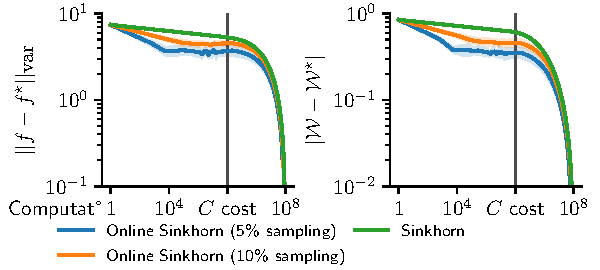
\includegraphics[width=.8\textwidth]{early_compute_low_eps.pdf}
    \caption{Online Sinkhorn accelerates the first Sinkhorn iterations even for low regularization. $\varepsilon = 10^{-4} \max C$.}
    \label{fig:early_compute_low_eps}
\end{figure}
